\newpage
\section{Screenshots}
\label{appendix:screenshots}

\begin{center}
	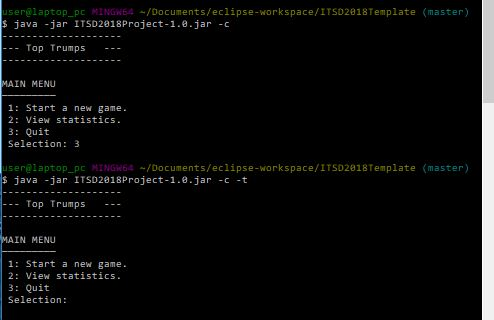
\includegraphics[scale=0.7]{S0010_GameInit}
	\captionof{figure}{Game Initialisation.}
	\label{figure:gameInit_true}
\end{center}
\begin{center}
	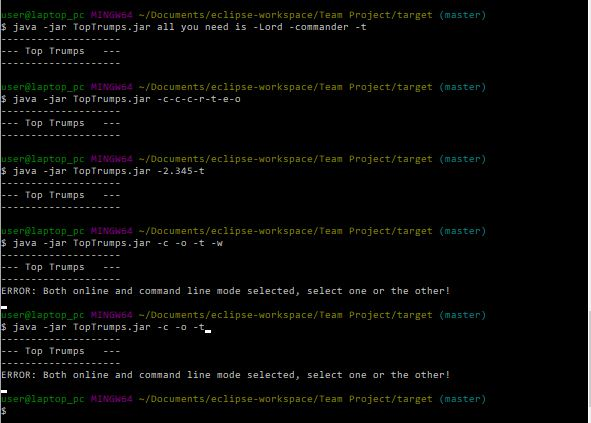
\includegraphics[scale=0.4]{S0010_GameInitAnti}
	\captionof{figure}{Game Initialisation with wrong flag.}
	\label{figure:gameInit_false}
\end{center}
\begin{center}
	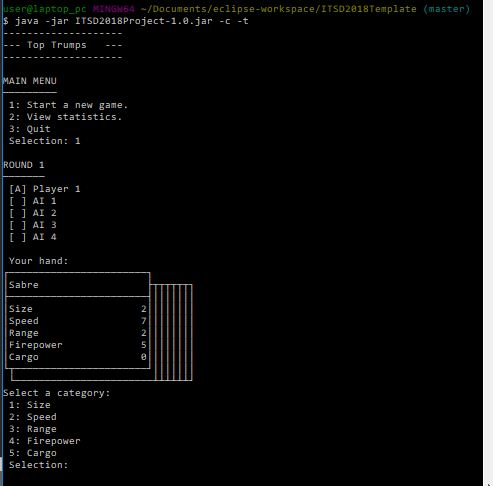
\includegraphics[scale=0.6]{S0010_MainMenu}
	\captionof{figure}{Main Menu with correct integer.}
	\label{figure:mainMenu_true}
\end{center}
\begin{center}
	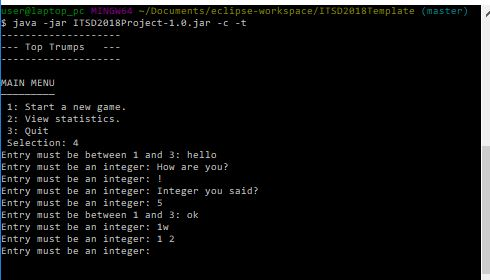
\includegraphics[scale=0.8]{S0010_MainMenuAnti}
	\captionof{figure}{Main Menu with incorrect integer.}
	\label{figure:mainMenu_false}
\end{center}
\begin{center}
	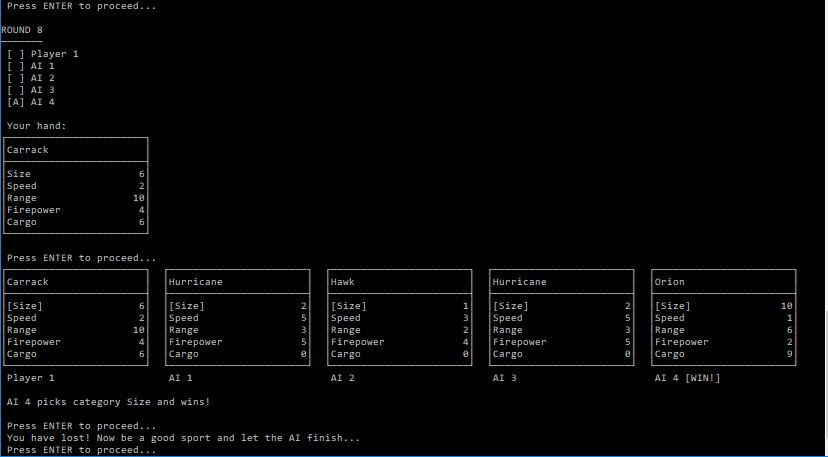
\includegraphics[scale=0.5]{S0030_S0040_RoundInfo}
	\captionof{figure}{Round information and human player is eliminated.}
	\label{figure:cmd_winner}
\end{center}
\begin{center}
	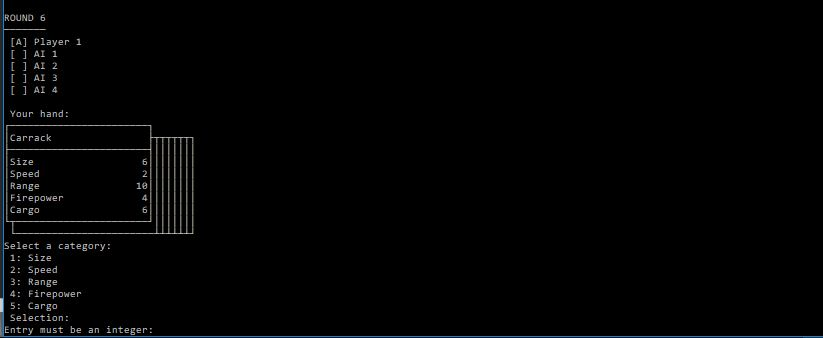
\includegraphics[scale=0.5]{S0030_HumanActive}
	\captionof{figure}{Human player is active player and has to select a category.}
	\label{figure:cmd_play}
\end{center}
\begin{center}
	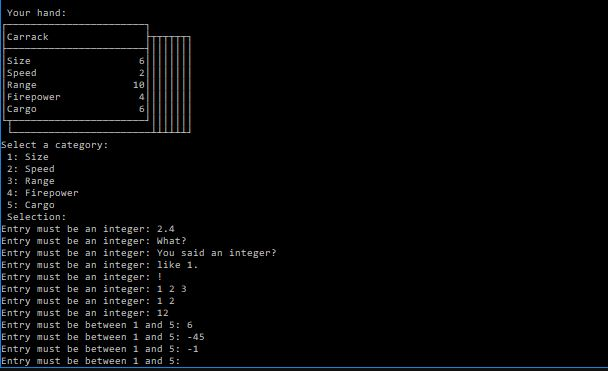
\includegraphics[scale=0.6]{S0030_WrongInput}
	\captionof{figure}{Human player is active player and enters wrong integer number.}
	\label{figure:falseInput}
\end{center}
\begin{center}
	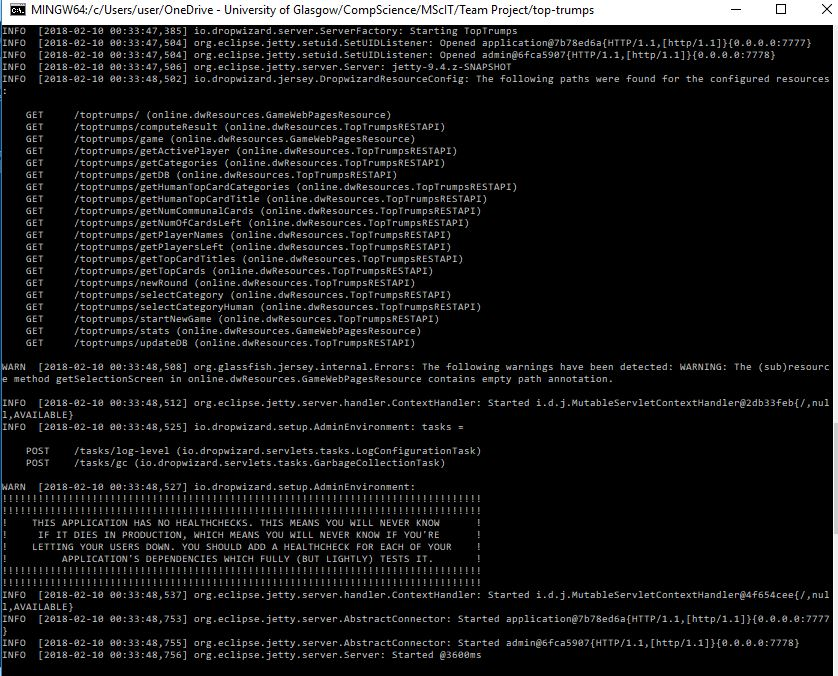
\includegraphics[scale=0.5]{S0200_OnlineMode}
	\captionof{figure}{Initialise online game mode.}
	\label{figure:onlineMode}
\end{center}
\begin{center}
	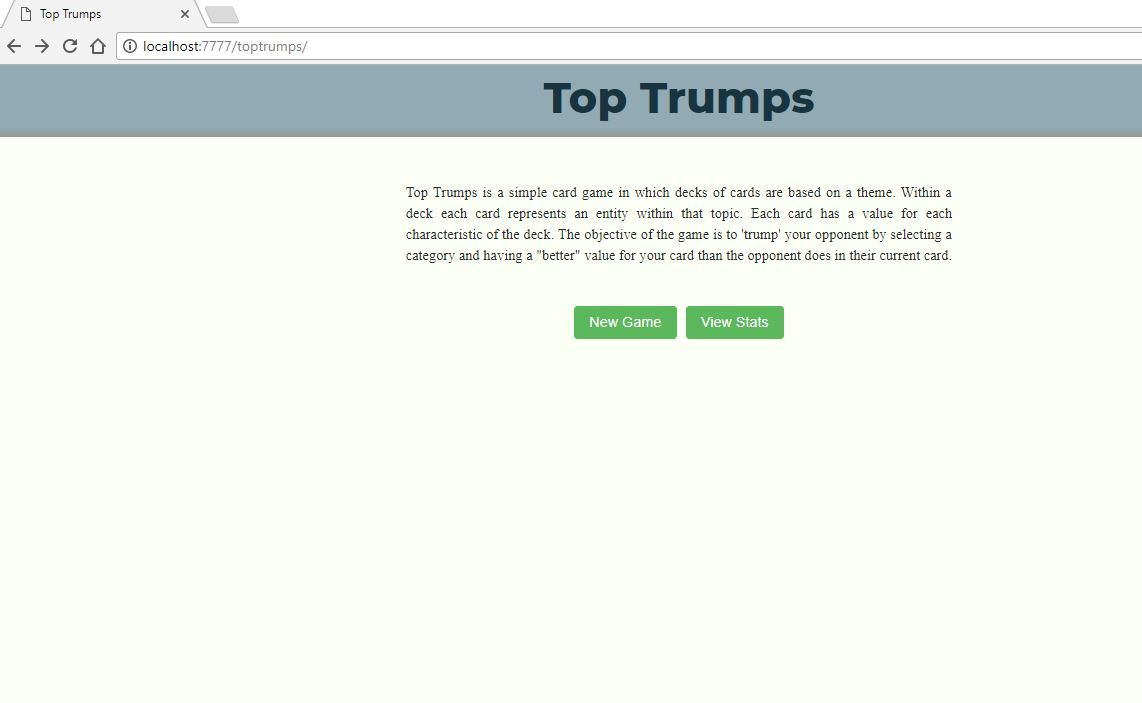
\includegraphics[scale=0.4]{S0200_MainMenu}
	\captionof{figure}{Main menu of the online mode.}
	\label{figure:online_menu}
\end{center}
\begin{center}
	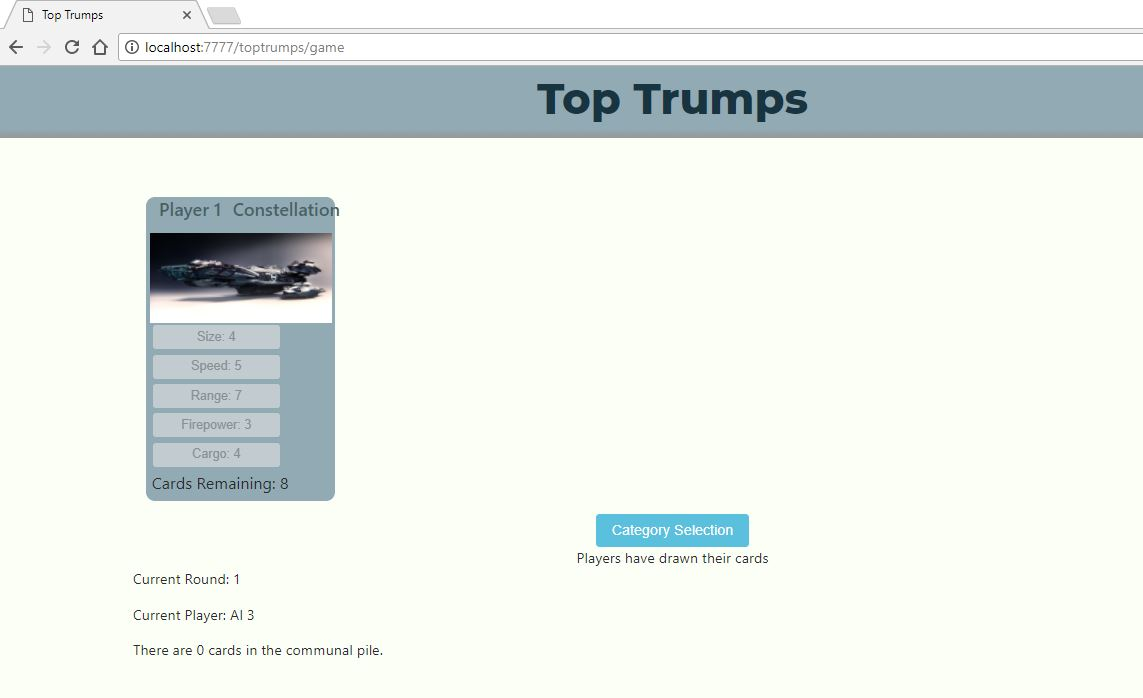
\includegraphics[scale=0.4]{S0220_RoundSet}
	\captionof{figure}{Initialised game, ready to start.}
	\label{figure:readyStart}
\end{center}
\begin{center}
	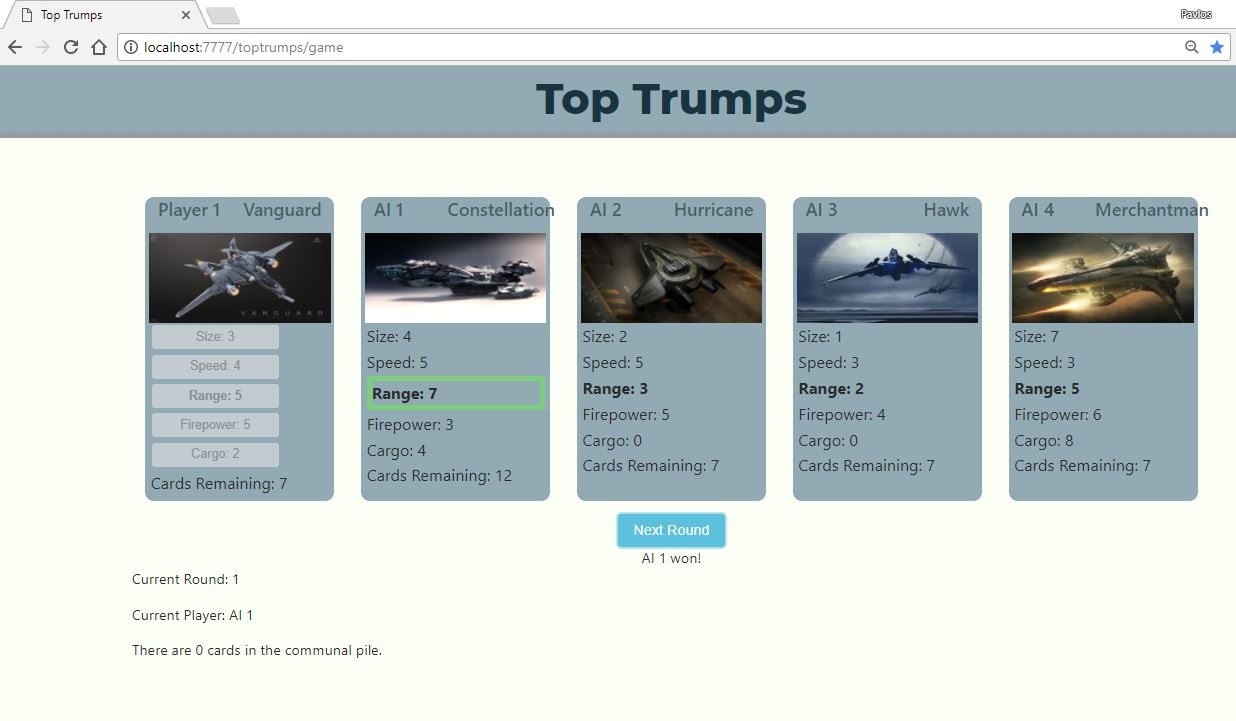
\includegraphics[scale=0.4]{S0220_RoundOutcome}
	\captionof{figure}{Round winner. With bold is the selected category and with the green rectangular indicates the winner}
	\label{figure:online_play}
\end{center}
\begin{center}
	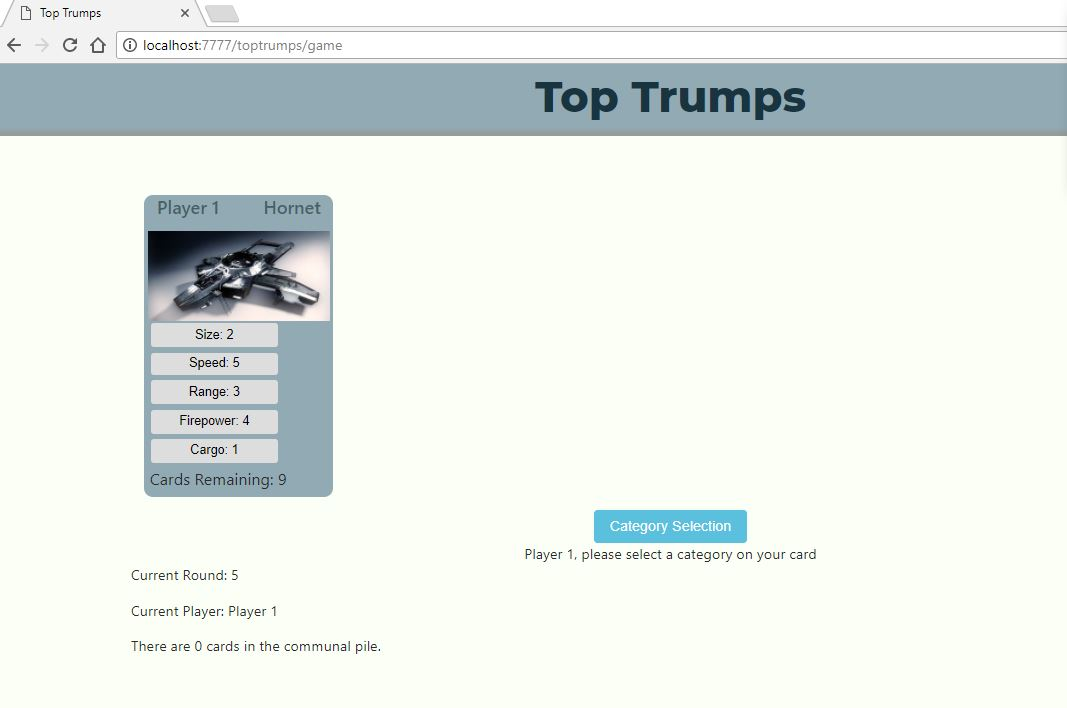
\includegraphics[scale=0.4]{S0220_selectCategory}
	\captionof{figure}{Round winner is the human player and must select a category before the game proceeds.}
	\label{figure:online_selectCategory}
\end{center}
\begin{center}
	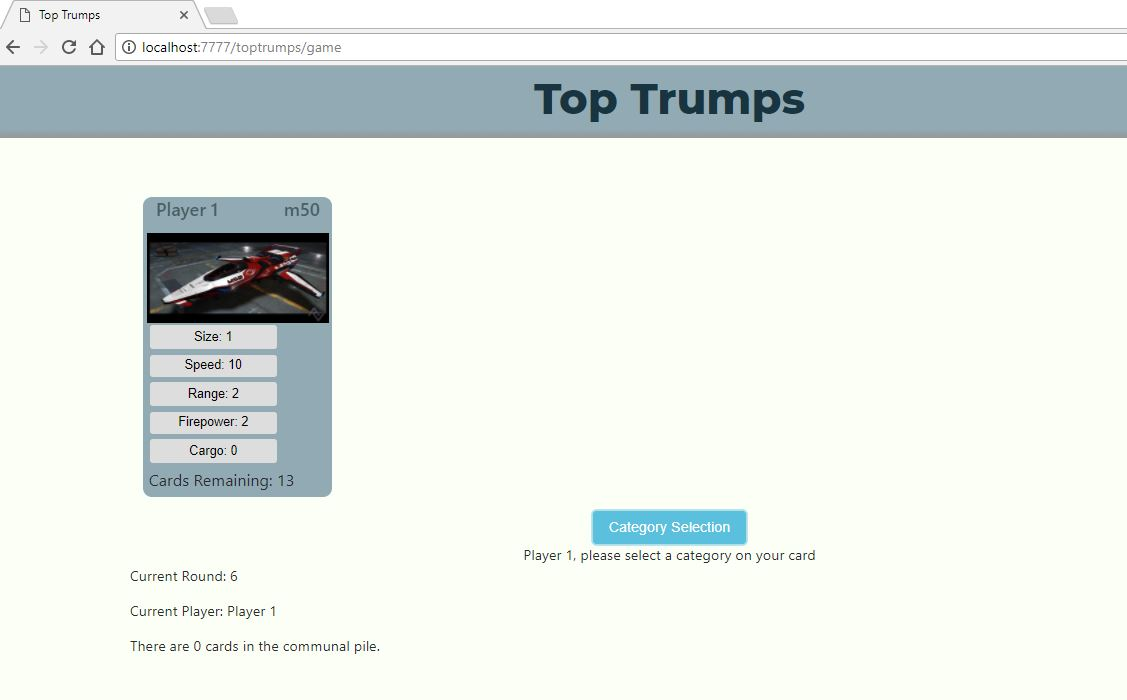
\includegraphics[scale=0.4]{S0230_HumanActive}
	\captionof{figure}{Below the main button displays the selected category and who was active player.}
	\label{figure:online_humanRound}
\end{center}
\begin{center}
	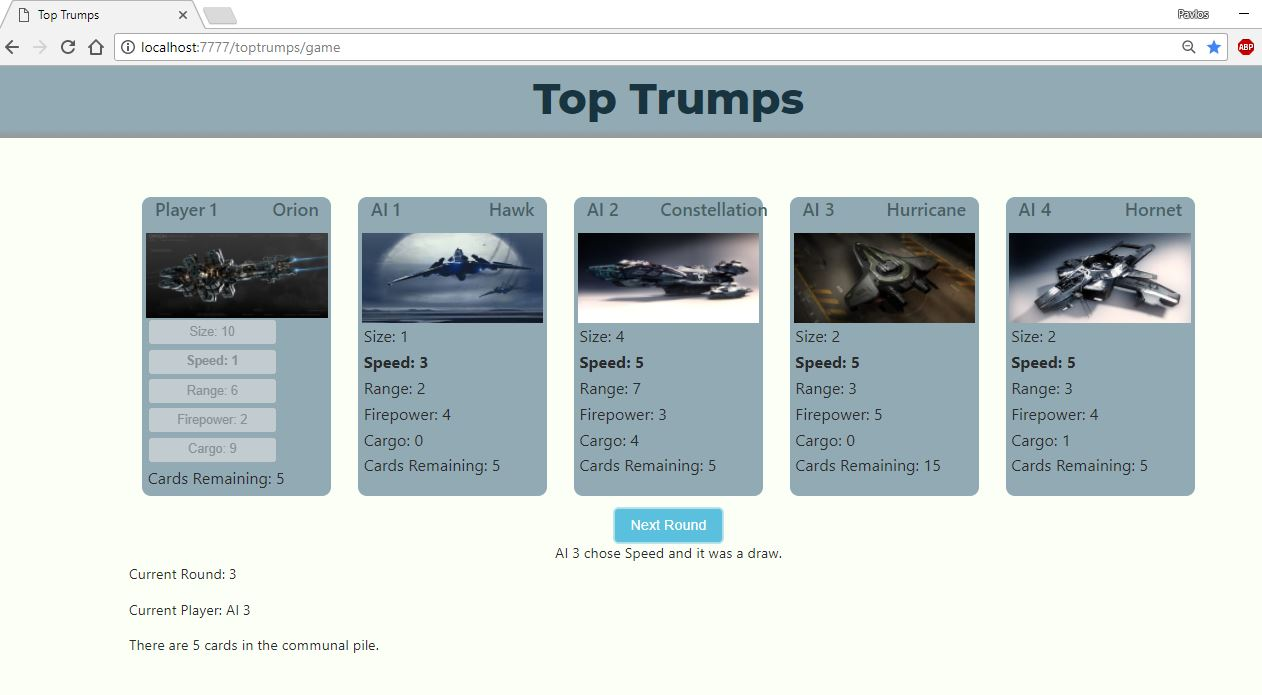
\includegraphics[scale=0.4]{S0240_DrawOnline}
	\captionof{figure}{Draw outcome. With bold is the selected category, there is no green indication of winner and the communal pile stores the cards of the players who are still in the game.}
	\label{figure:drawOnline}
\end{center}
\begin{center}
	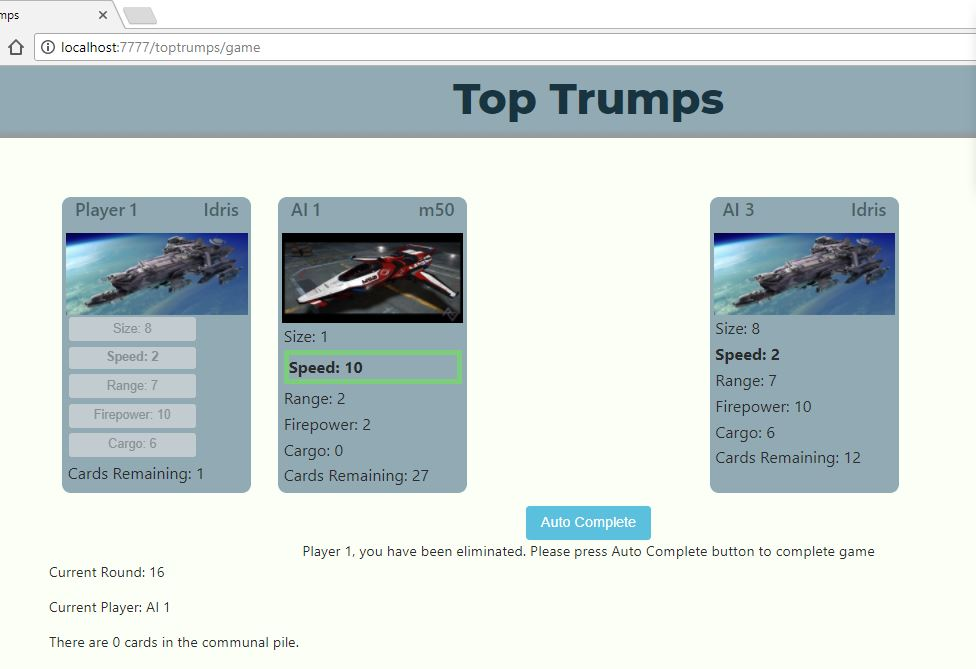
\includegraphics[scale=0.4]{S0250_AutoComplete}
	\captionof{figure}{If the human player is eliminated the auto-complete button appears.}
	\label{figure:autoComplete}
\end{center}
\begin{center}
	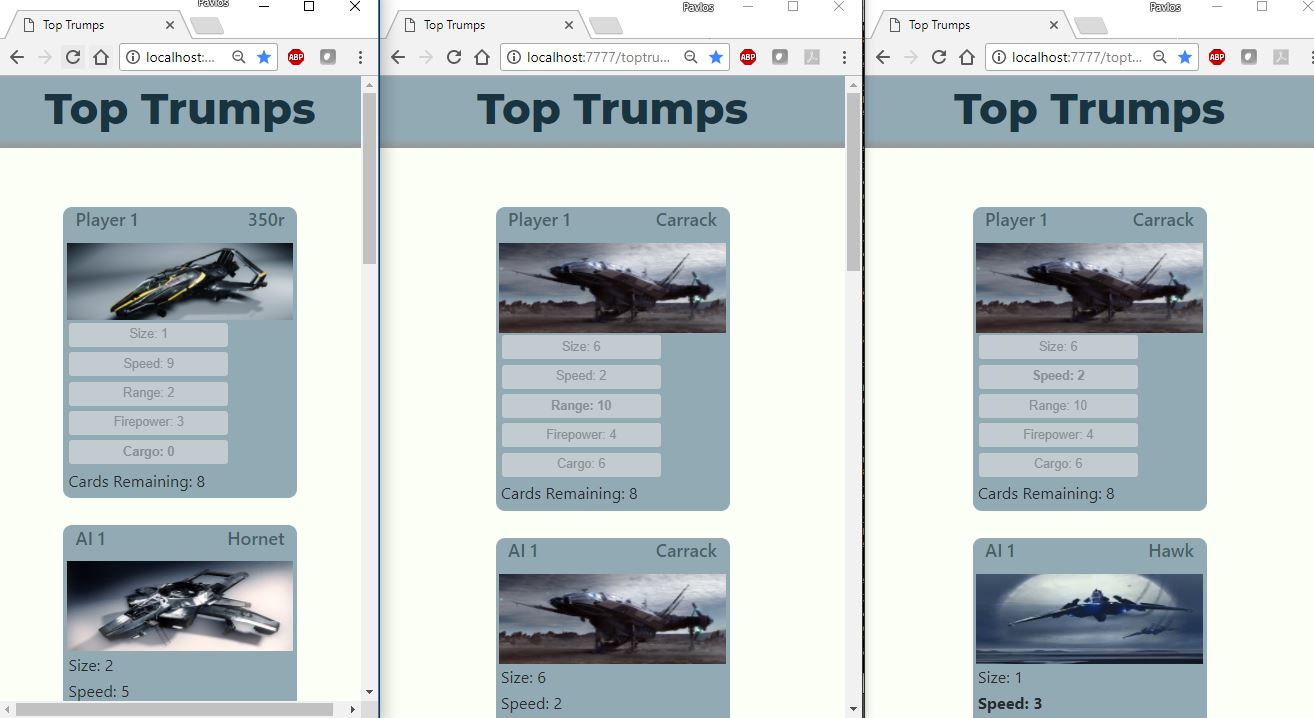
\includegraphics[scale=0.4]{S0250_MultipleGames}
	\captionof{figure}{Multiple games can exist simultaneously in different tabs with game index.}
	\label{figure:multipleGames}
\end{center}
\begin{center}
	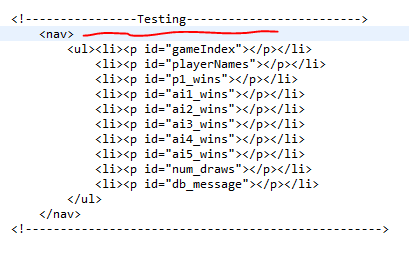
\includegraphics[scale=0.5]{onlineTesting}
	\captionof{figure}{The above variables were not hidden during the development of the, in order to test the functionality of the online mode.}
\end{center}
\begin{center}
	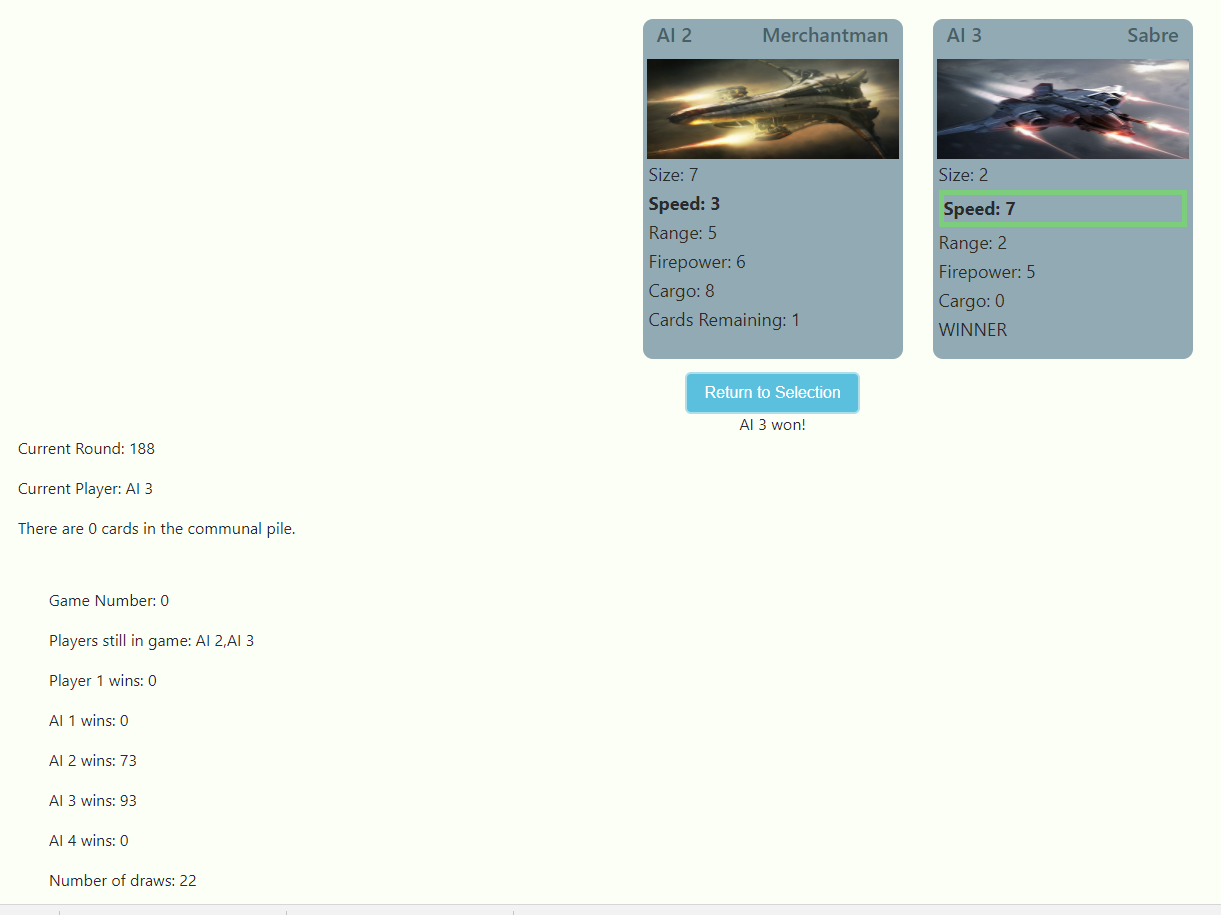
\includegraphics[scale=0.3]{onlineTesting_2}
	\captionof{figure}{This figure is connected with the figure above and provides a clear understanding about the testing.}
\end{center}
\begin{center}
    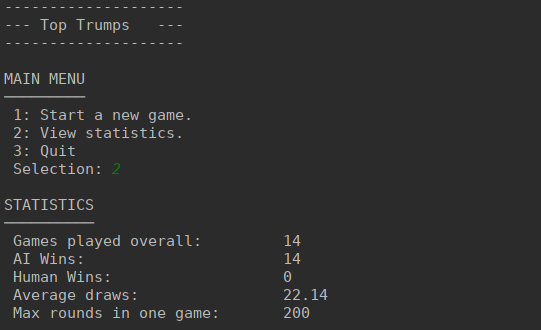
\includegraphics[scale=0.7]{cmd_stats}
    \captionof{figure}{Command Line Statistics View}
    \label{figure:cmd_stats}
\end{center}
\begin{center}
    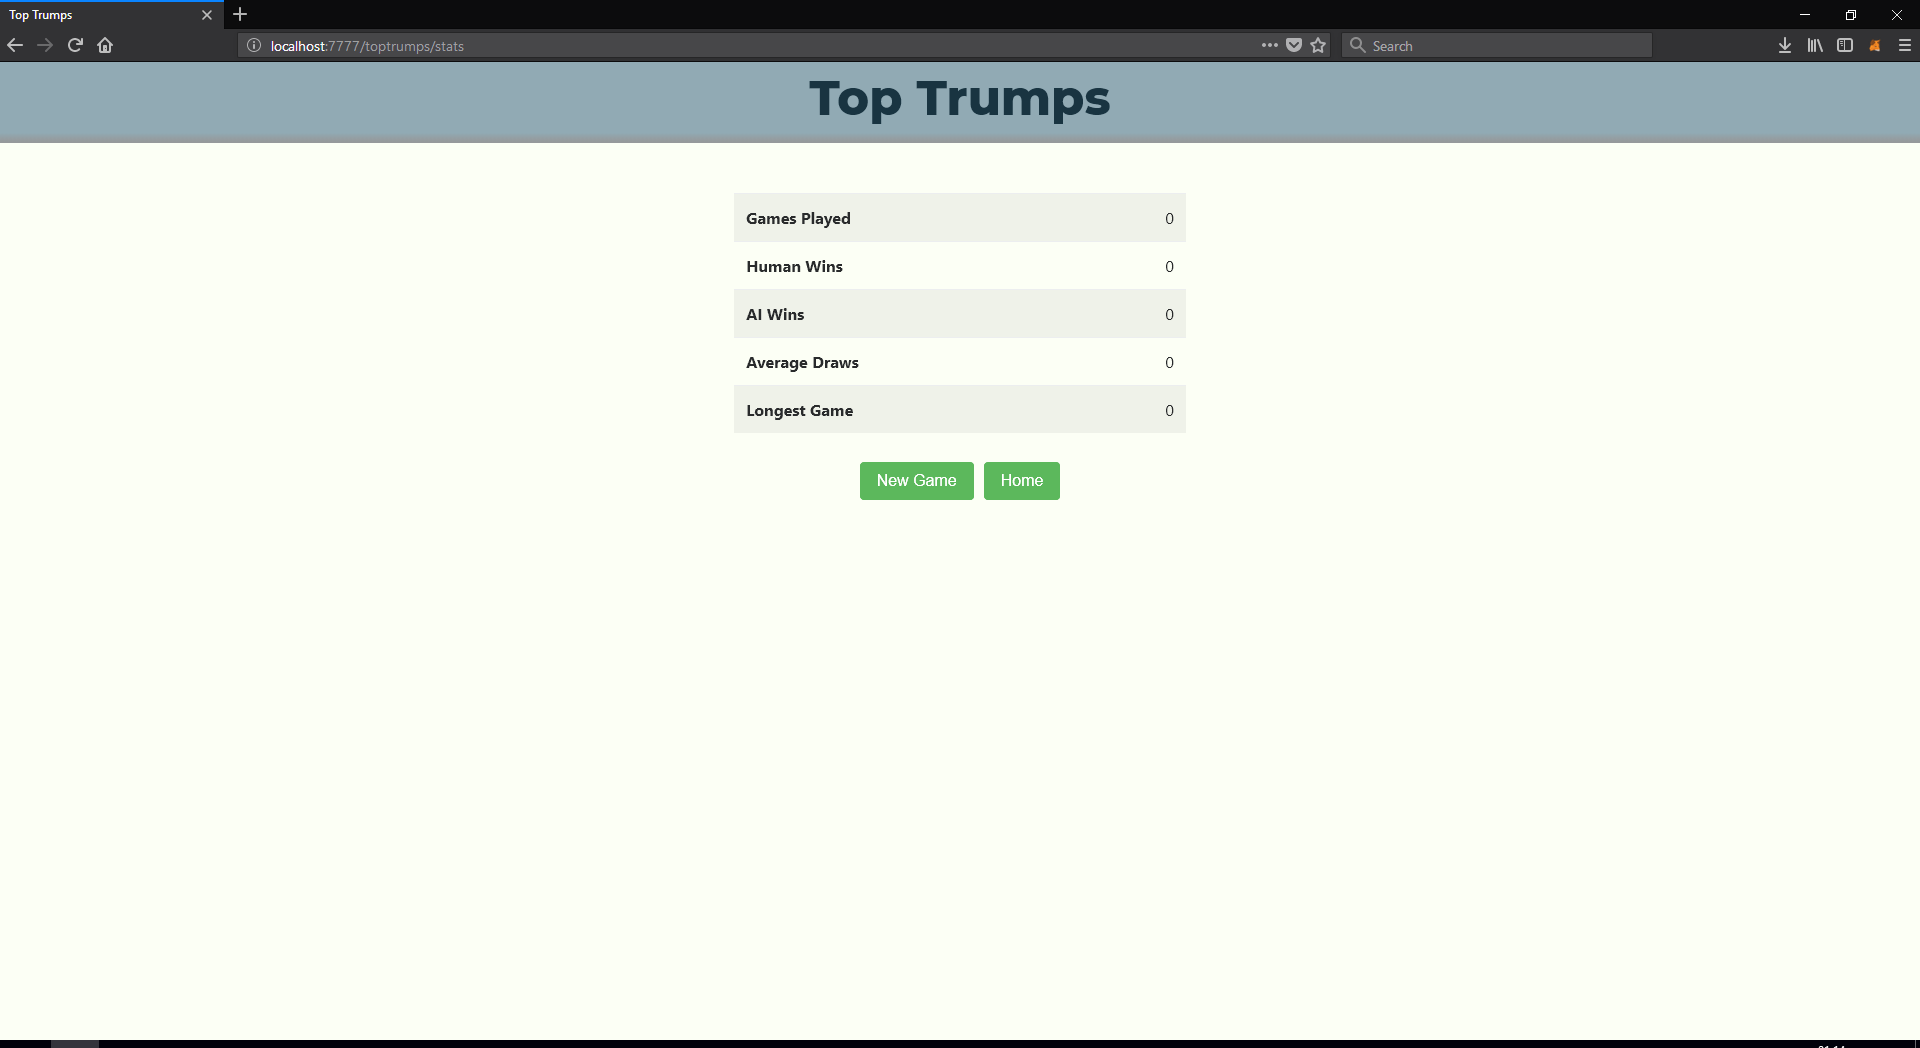
\includegraphics[width=\textwidth]{online_stats}
    \captionof{figure}{Online Statistics View}
    \label{figure:online_stats}
\end{center}
\begin{center}
    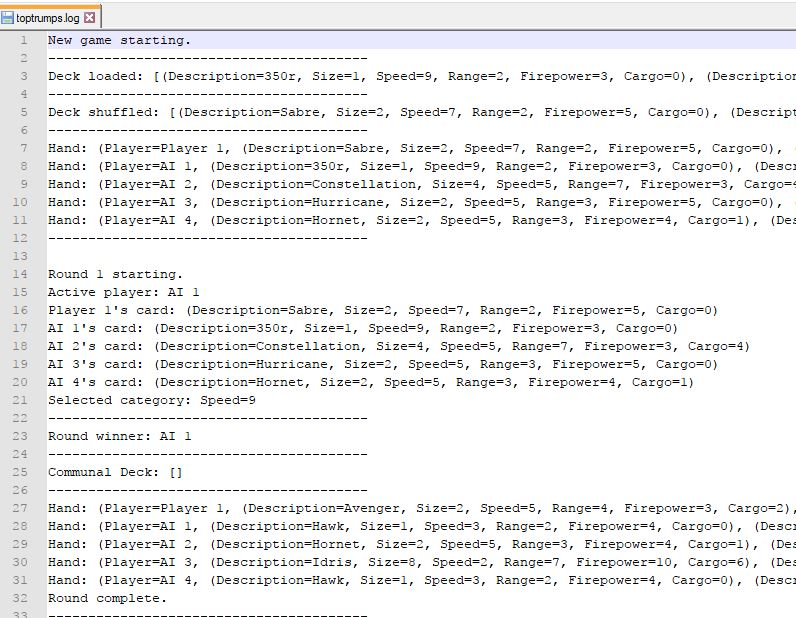
\includegraphics[scale=0.6]{S0020_testlog}
    \captionof{figure}{All the details of the game is inside the test log file.}
    \label{figure:testlog}
\end{center}
\begin{center}
    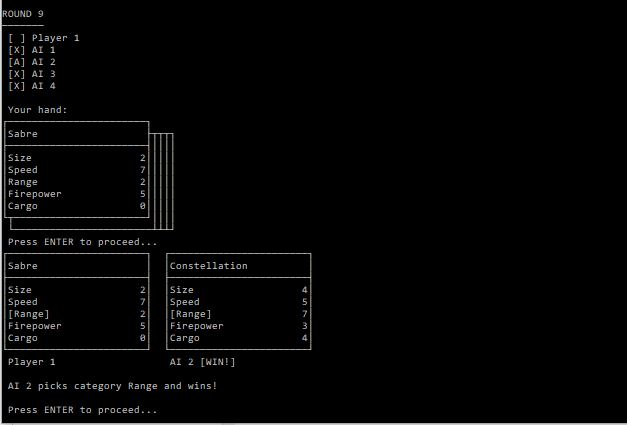
\includegraphics[scale=0.7]{S0050_showEliminated}
    \captionof{figure}{The program shows who is eliminated from the game with a X mark inside the brackets.}
    \label{figure:eliminated}
\end{center}

